\documentclass{TDP003mall}
\usepackage{listings}
\usepackage{xcolor}


\newcommand{\version}{Version 2.2}
\author{Arturas Aleksandrauskas\\
  Joakim Johansson}
\title{Systemdokumentation}
\date{2016-10-18}
\rhead{Arturas Aleksandrauskas\\
Joakim Johansson}



\begin{document}
\projectpage

\tableofcontents

\newpage
\section{Revisionshistorik}
\begin{table}[!h]
\begin{tabularx}{\linewidth}{|l|X|l|}
\hline
Ver. & Revisionsbeskrivning & Datum \\\hline
2.2 & Autogenererat dokumentation utifrån filernas kommentarer och lagt in & 161017 \\\hline
2.1 & Lagt till mer kommentarer i filerna & 161017 \\\hline
2.0 & Börjat fixa kompletteringarna & 161017 \\\hline
1.5 & Logging, Error handling och Tools inlagt och första utkast inlämnat & 161016 \\\hline
1.4 & Description of the system components - Datalagret är första utkast inlämnat & 161016 \\\hline
1.3 & Description of the system components - Presentationssidan är klart & 161015 \\\hline
1.2 & User Functions och Folder Structure sectionerna är skrivna tillagda & 161015 \\\hline
1.1 & Skissat och lagt till sequensdiagram och skrivit klart Overview of the system och Frontpage exemplet & 161014 \\\hline
1.0 & Dokumentet skapas och enkel information har lagt in som en start, A simple description och Installationsmanual är tillagt och klart & 161012 \\\hline
\end{tabularx}
\end{table}

\section{A simple description}
This project is made up by a basic backend which is a python file using the flask module to listen and answer to HTTP-requests.

The purposes of this website i to present a list of all projects the user has previously been involved in. A visitor of the site can scroll though all, or search for a specific project.\\

\section{Installation manual}
If you got this system documentation file, you have probably also got a separate PDF file that is the Installation manual. Use that if you are going to install the system om a new computer.\\

In case you haven't got the PDF, here is the link to an online version:

\url{https://gitlab.ida.liu.se/antsu07/tdp003-installationsmanual-2016/blob/master/installationsmanual.pdf}



\newpage
\section{User Functions}
The user will we able to go to four different pages.\\


\includegraphics[width=\textwidth]{bilder/headerandnav.png}\\

On the top of the webpage there is a header with the name of the website, which the user always will be able to click on to go back to the front page. This way, if the user gets lost on the site, he can just click the logo and be directed to home again.\\

Under the header, there is a navigation bar with two links. The List page and the Technologies page. This navigation bar with be easily accessible from all pages on the site.\\

The first page is a simple front page that displays useful about-information about the websites author. The page also displays all the three latest projects. Visitors can of course click on the projects to show more information.\\


\includegraphics[width=\textwidth]{bilder/search.png}

The second page is the List page, which the user can get to by clicking in the navigation bar or searching from the 404 error page. The list page is made up of a long list of all projects in the database. There is also a box of tools filter the list. Visitors can search with free-text, choose required techniques, and choose how the list should be ordered. And of cause there is a search button to apply the filters to the list.\\

The third page is the Technologies page. This is more of a overview over all projects with the techniques in focus. This page is great for visitors to quickly see what type of techniques the author uses most. But it is also really handy when a visitor looks at a project that uses ex. python and want to now other project the author have done where he also has used python.\\

The fifth page is a page that only shows a specific project. This page is hidden in the menu and you can only get to the page if you click on a project somewhere. This page shows a lot of information about the project, ex. the techniques used, start and end date, peoples in the project and more. If the visitor clicks on a technique, he will be directed to the technique page and moved down to the right place for the clicked tech.\\

The last page we have are the error page, it's displayed if the user tries to go to a page that don't exist. Simple as that. The page as a title, a short text and a search box so that the user can continue trying to find the right page.\\



\newpage
\section{Folder structure with description of the files}

\begin{lstlisting}[backgroundcolor=\color{lightgray}]
.
  Root/
      doc/
      static/
          images/
          style/
              style.css
      templates/
          index.html
          list.html
          project.html
          technologies.html
          error.html
      README.md
      data.json
      data.py
      data_test.py
      myFlaskProject.py
      logfile.log
.
      
\end{lstlisting}

\subsubsection{Folder: doc}
A folder with all documents related to this project but isn't actually code, like this document for example.\\

Here, you can also find the project plan document, LoFi prototype and the developers diary if you want to follow the development.

\subsubsection{Folder: static}
A folder with all the static files, like CSS, images and fonts.\\

We have no images yet, but we have added a folder in case we want to do future graphical enhancements to the site. We also have a folder called style. It has a single CSS file inside it that is used to style all pages.\\

\subsubsection{Folder: templates}
A folder for all the HTML templates.\\

We user five templates. One for each page on the site. index.html for the front page, list.html for the list page, project.html for the page that shows one project, technologies.html for the page with all the projects sorted by tech and error.html for the error page.

\subsubsection{File: README.md}
A description file with info about the project and good information for outside people in case they open up this project and don't know what it is.

\subsubsection{File: data.json}
Our main database name with all data from all the projects. Used by the API.

\subsubsection{File: data.py}
This is the API-side of the project. Gets imported by the flask file and is used on almost every HTTP request.

\subsubsection{File: data\_test.py}
This is a test file that is used to test the data.py file so that it is ok on all the requirements made up by the university.

\subsubsection{File: myFlaskProject.py}
This is the main flask file that is active running on the server and waiting for HTTP request to handle. If a request appears, the script goes to the function handling that request, contacts the API, does some calculations and at the end, returns a HTML-page.

\subsubsection{File: logfile.log}
This is the log file that is created by flasks and contain all logs and actions that flask have done.




\newpage
\section{Overview of the system}
The system is a basic system for handling some webpage requests and some data.\\

It's made up of a client side and a server side. The client side is simply the users browser, with the functions of requesting a page using the GET method.\\

The server side is made up of two main processes, the python flask webserver file and the API file that handles all the data. The API file uses a JSON file to store all the information.\\

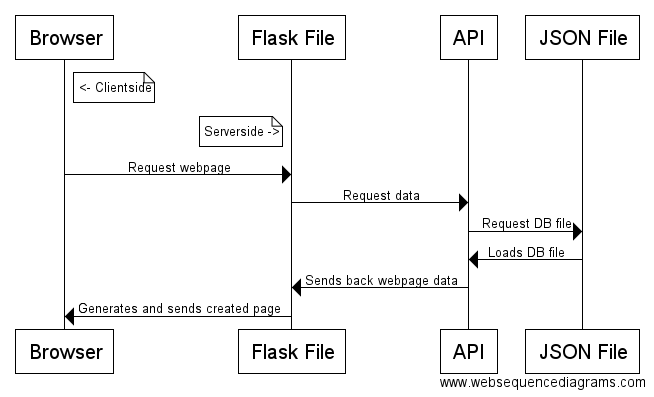
\includegraphics[width=\textwidth]{bilder/diagram_overview.png}




\newpage
\subsection{Example Scenario - Front page}
When the user goes to the root of the webpage, the browser sends a request to the the server where flask is waiting and have a function bind to requests for the root directory. In this case, the hello() function is run. Hello() does two things, requests the database file from the API and then sends it back to the API layer with the request that it should search and filter the database object. In this case we only the send the database as a parameter to get all the latest projects with the newest projects first, but we could specify multiply parameters to tell the search function how it should filter the projects.\\

When the Flask layer get the filtered data, it imports the HTML templates, CSS files and other static files like images. Then it generates the HTML-files from the templates and the filtered data, and finally sends it back to the users browser that displays the webpage to the user.\\

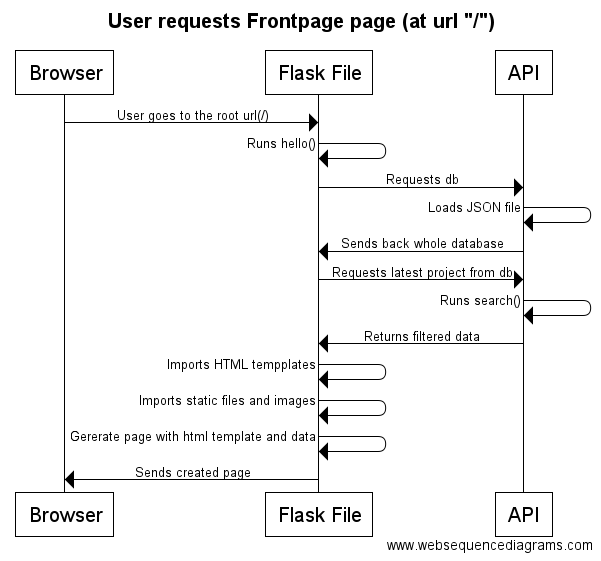
\includegraphics[width=\textwidth]{bilder/frontsida.png}




\newpage
\section{Description of the system components}

\subsection{Client Browser}
The client side simply request a webpage using GET and renders the HTML, CSS and JavaScript’s that it get as return value.

We use the latest HTML5 and CSS3. If the link ends with a #word, the client’s browser will scroll down to the position where there are a HTML-element with the id #word.

\subsection{Flask Webserver}
\subsubsection{hello()}
    Handling requests for the index page. Returns a html page with some CSS.
    This function loads the all data thought the API and uses the search-function of the API to filter out the latest projects.
    Uses the ninja function render\_template to combine the filtered projects with the html-page and sends it back to the client.\\

    Input:\\
    Output: Index.html with data about the three latest projects\\
\subsubsection{techniques()}
    Handling requests for the technologies page. Returns a html page with some CSS.
    This function loads the all data thought the API and uses the get\_technique\_stats-function of the API that returns all project stats for the tech page.
    Uses the ninja function render\_template to combine the tech-data with the html-page\\

    Input:\\
    Output: technologies.html with data about every technique and it's projects\\
\subsubsection{list()}
    Handling requests for the list page. Returns a html page with some CSS. Uses the method GET.
    
    This function does two things. First it requests a list of all techniques from the API, just to create a dropdown with all the techniques on the finished page.
    This function loads the all data thought the API and uses the get\_techniques-function of the API that returns a list of all techniques for the checkboxes on the page.\\
    
    But the main thing about this function is that it loads the database file (though the API) and then sends it to the search function of the API together with a lot of parameters that is created if the user submitted the form on the list page.\\
    
    It also has some self-explanatory code for auto filling the page on load so the user does not have to retype the search key between every page load.\\

    At the end, it uses the ninja function render\_template to combine the data from the API:s search function with the html-page and sends it back to the client.\\

    Input:\\
    Output: list.html with the search data\\
\subsubsection{project(xid)}
    Handling requests for the project page. Returns a html page with some CSS. This function uses the id-number form the URL request.
    This function loads the all data thought the API and uses the get\_project-function of the API that returns the required project.
    Uses the ninja function render\_template to combine the data with the html-page
    Also has some error handling for is the types a unexpected id in the URL, the it renders the error page instead of the regular page.\\

    Input: ID for the project\\
    Output: project.html with data about the project\\
\subsubsection{error(e)}
    Handling error requests and uses the ninja function render\_template to render the error.html page with some information about the error. There is also a search box on the page so the user can continue searching the wanted page and not give up.\\

    Input: e which is information about the error\\
    Output: error.html with data about the error\\

\subsection{Data layer / API}
This component of the system has been create with the requirements from the course leader in mind.

\url{ http://www.ida.liu.se/~TDP003/current/portfolio-api_python3/}

\autocite{\footnote{\url{ http://www.ida.liu.se/~TDP003/current/portfolio-api_python3/}}:2016}

\subsubsection{load(file\_json)}
  Tries to load a file with the provided name. If success it returns the file in JSON format, it not, it returns none.\\

  Input: A filename (string)\\
  Output: All project (dictionary)\\

\subsubsection{get\_project\_count(db)}
  This function takes in a database object and returns amount of project in that database.\\

  Input: A database (dictionary)\\
  Output: Amount of projects (int)\\

\subsubsection{get\_project(db, id)}
  Returns all the information about the project with the provided id.\\

  Input: A database (dictionary), ID (int)\\
  Output: A dictionary with information about the project\\

\subsubsection{search(db, sort\_by='start\_date', sort\_order='desc', techniques=None, search=None, search\_fields=None)}
  Handling a search request.
  Creates an empty temporary list.
  Filters out all projects that has the right search text in the right search fields.
  Filters out all projects with the right techniques.
  Then some code for selecting order.
  Sorts the projects left.
  Returns the projects that passed thought the filters.\\

  Input: A database (dictionary), order by field (string), sort order (string), list with techniques (list), search text (string), search fields to sort in (list)\\
  Output: A database dictionary with only the projects that made it though the search requierments\\

\subsubsection{get\_techniques(db)}
  Returns a sorted list of all techniques in the provided database object.\\

  Input: A database (dictionary)\\
  Output: A list of all techniques in the database\\

\subsubsection{get\_technique\_stats(db)}
  This function creates a custom dictionary from the provided database object. The dictionary is made so that the name of the technique is the key of every item and the value is a list with project objects using that technique. Then it returns the custom list with techniques and its projects.\\

  Input: A database (dictionary)\\
  Output: A dictionary with all techniques as keys and the value for each key is a list of projects that has that specific tech (each project is a dictionary with a id and a name key)\\

\subsubsection{search\_in\_search(projects\_left, search\_fields, search, item, project)}
  This is a help function for the search\_search\_fields function. It checks if the search text is in the selected fields. Used the search\_search function as help.\\

\subsubsection{search\_search(value, search)}
  This is a help function for the search\_in\_search function. It returns true or false, based on if a specific spot in the search text matches any text in the search field.\\

\subsubsection{search\_search\_fields(db, projects\_left, search\_fields, search)}
  This is a help function for the search\_search function. 
  Checks if the search text is in the search fields. Used the search\_in\_search function.\\

\subsubsection{search\_techniques(projects\_left, tech)}
  This is a help function for the search function. 
  Filters out the project that uses a specific technique.\\


\newpage
\section{Others}

\subsection{Logging}
Flask is setup in a way that it should log every action that happens in a log file in the root directory named logfile.log. The log file is located in the root directory.

\subsection{Error handling}
The website redirects the user to the error page in case they try to go to a URL that is not valid.\\

If you want to enable debug mode in flask, simply add debug=true as a parameter in the app.run(). You will then be able to see every action in the terminal and you will also be able to edit the files and see the change on the page without restarting the server.

\subsection{Tools and programs}
To compile all the documents in the doc folder, you have to use a latex compiler to export a PDF from the code. On Linux, we recommend using the command latexmk -pvc -xelatex and then the filename of the .tex file of the wanted document. But there is usually an already compiled PDF file in the related folder ready for use.



\end{document}





